% !TEX root = ../thesis.tex

%%%%%%%%%%%%%%%%%%%%%%%%%%%%%%%%%%%%%%%%%%%%%%%%%%%%%%%%%%%
% Chapter: Aspect refactoring 
%%%%%%%%%%%%%%%%%%%%%%%%%%%%%%%%%%%%%%%%%%%%%%%%%%%%%%%%%%%
\chapter{Aspects refactoring of JHotDraw}\label{AspectRefactoring}

\section{JHotDraw And AJHotDraw}\label{JHotDraw And AJHotDraw}
JHotDraw\footnote{\url{http://www.jhotdraw.org/}} is a Java GUI framework for technical and structured graphics. 
It is an open-source, well-designed and flexible drawing framework of around 18,000 non-comment lines of Java code. 
JHotDraw's  design relies heavily on some well-known design patterns \cite{gamma1995design} and it is considered as a showcase for software quality techniques provided to the \ac{oop} community. 

The fact that JHotDraw is praised for its design makes it an ideal candidate as a showcase for an aspect oriented migration. 
Marin and Moonen \cite{marinajhotdraw} use this showcase for adoption of aspect-oriented techniques in existing systems. 
In particular, they present AJHotDraw\footnote{\url{http://swerl.tudelft.nl/bin/view/AMR/AJHotDraw}}, which is an aspect-oriented version of JHotDraw developed in Java and AspectJ. 
The goal of AJHotDraw is to take JHotDraw and migrate it to a functionally equivalent aspect-oriented version. 

The authors presented a fan-in analysis of JHotDraw \cite{marin2004identifying} and implemented an idiom-driven approach to aspect-mining. 
This way they could extract a number of aspects in JHotDraw. 
Next, they performed a concern exploration in order to expand their mining results, leading to concern sorts.
Concern sorts is a consistent way to address crosscutting concerns in source code \cite{marin2005classification}.
This led to the identification and documentation of \ac{ccc} in JHotDraw, which helps the developers to identify \ac{ccc} in it.
In order to handle the aspects in a more consistent and formal way, Marin et al. provided a list of \textit{template aspect} solutions for their concern sorts.
Finally, they performed aspect refactoring of JHotDraw by presenting the AJHotDraw, which according to them, was the largest migration to aspects available to date.
Their refactoring aimed at maintaining the conceptual integrity of the original design.

In order to refactor the existing framework, the first thing that AJHotDraw developers needed to do was to create a test subproject for the JHotDraw, called TestJHotDraw\footnote{\url{http://swerl.tudelft.nl/bin/view/AMR/TestJHotDraw}}, which ensures behavioral equivalence between the original and the refactored solution. 
Refactoring implies preserving the observable behavior of an application \cite{fowler2009refactoring} and since the developers of AJHotDraw ought to test their functionality, TestJHotDraw was created. 
There are several contributions of the aspect-oriented implementation approach \cite{marinajhotdraw}. 
The authors suggest that the project contributes to a gradual and safe adoption of aspect-oriented techniques in existing applications and allows for a better assessment of aspect orientation.

In this thesis we have used JHotDraw and AJHotDraw in order to evaluate our aspect refactoring in managed data.
However, TestJHotDraw is written in AspectJ, a language we did not want include in our project, and therefore it is not used.
Instead, we used the JHotDraw original test suite, which consists of 1218 test cases, for our refactoring behavioral preservation.

%%%%%%%%%%%%%%%%%%%%%%%%%%%%%%%%%%%%%%%%%%%%%%%%%%%%%%%%%%%
\subsection{Refactoring of Crosscutting Concerns}\label{Refactoring of ccc}
The refactoring of legacy code to aspect oriented code is also known as \textit{Aspect Refactoring} \cite{marin2005approach}. 
During this process it is important to identify which elements are going to be refactored and which \textit{aspect} solutions will replace them. 
To evaluate the refactored elements \cite{fowler2009refactoring}, a testing component is needed in order to ensure behavior conservation, hence some coherent criteria to organize \ac{ccc} are needed. 
% Marin, Moonen and Deursen \cite{marin2005approach} organize the \ac{ccc} into types, which are descriptions of similar concerns that share the following properties: 

% \begin{itemize}
% 	\item A generic behavioral, design or policy requirement to describe the concern within a formalized, consistent context (e.g., role superimposition to modular units (classes), enforced consistent behavior, etc.),

% 	\item An associated legacy implementation idiom in a given (non-aspect oriented) language (e.g., interface implementations, method calls, etc.)

% 	\item An associated (desired) aspect language mechanism to support the modularization of the type's concerns (e.g., \texttt{pointcut} and \texttt{advice}, introduction, composition models).
% \end{itemize}

%%%%%%%%%%%%%%%%%%%%%%%%%%%%%%%%%%%%%%%%%%%%%%%%%%%%%%%%%%%
% \subsection{The Observer Pattern}\label{The Observer Pattern}
% As discussed, design patterns introduce \ac{ccc} by scattering ``pattern code'' through an application.
% Hannemann et al. \cite{hannemann2005role} discuss this with an example of \ac{ccc} refactoring of the observer pattern.

% \subsubsection{Role-based Refactoring}

\subsection{Role-based Refactoring}
Marin, Moonen and Deursen \cite{marin2005approach} present a \textit{role-based} refactoring, which consists of classifying the roles of the pattern in different aspects.
The role-based refactoring approach helps the developer to transform a scattered implementation of \ac{ccc} into an equivalent but modular \ac{aop} implementation. 
Both \ac{ccc} and refactoring are described in terms of roles. 

According to the authors \cite{hannemann2005role}, the steps of role-based refactoring are the following:
\begin{description}
	\item [Selecting a \ac{ccc} refactoring:] The refactoring includes an abstract description of the \ac{ccc} it targets and a set of instructions to produce a modular AOP implementation of the refactoring (e.g. the Observer pattern \ac{ccc} refactoring).

	\item [Stating a mapping:] Map role elements comprising the \ac{ccc} description to the program elements of the scattered code (e.g. the Subject and the Observer role to concrete classes)

	\item [Planning the refactoring:] make the right choices for specific cases since a \ac{ccc} refactoring involves modifying several parts of a codebase (e.g. naming).

	\item [Execution:] transform the code according to the refactoring instructions (e.g. modularizes Observer pattern as a result).
\end{description}

Thus, to refactor \ac{ccc} it is required a mapping from the abstract \ac{ccc} description to programming components that explicitly describe the \ac{ccc} implementation.
% This mapping for the case of the observer pattern is presented in Figure \ref{fig:Observer_Role_Mapping}.

% \begin{figure}[H]
% 	\centering
%   	\fbox{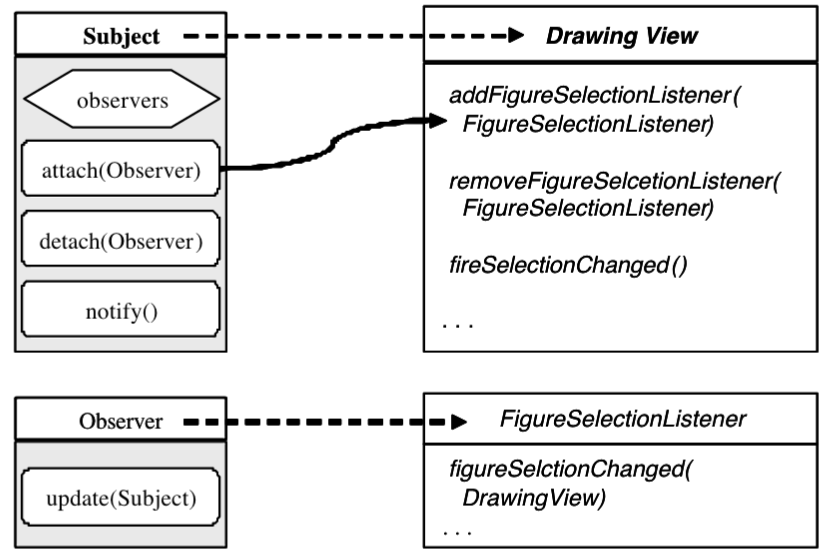
\includegraphics[width=.50\textwidth]{figures/observer_pattern_role_mapping.png}}
%   	\caption{Observer pattern: Role Mapping \cite{hannemann2005role}}
%   	\label{fig:Observer_Role_Mapping}
% \end{figure}

% This figure describes the roles mapping in a specific case on JHotDraw, the \textit{Figure Selection Listener}.
% However the authors have shown an abstract and reusable way of describing those roles.

% %%%%%%%%%%%%%%%%%%%%%%%%%%%%%%%%%%%%%%%%%%%%%%%%%%%%%%%%%%%%%%%%%%%%%%%%%%%%%%%
% \subsection{The Figure Selection Observer of JHotDraw}\label{The Figure Selection Observer of JHotDraw}
% % As mentioned above, Hannemann et al. \cite{hannemann2005role} presented a refactoring of the \textit{Observer} design pattern in JHotDraw.
% During the AJHotDraw implementation\cite{marin2005approach}, the authors proposed a type-based refactoring on the same \textit{Observer} instance, as Hannemann did \cite{hannemann2005role}, the \texttt{FigureSelectionListener}.

% The concern sorts identified in this case are: the \textit{Role Superimposition}, which is similar to the role-based refactoring described previously and the \textit{Consistent Behavior}, which describes a set of methods consistently invoking a specific action as a step in their execution.

% The legacy design of JHotDraw is displayed in Figure \ref{fig:Selection_Listener}.

% \begin{figure}[H]
% 	\centering
%   	\fbox{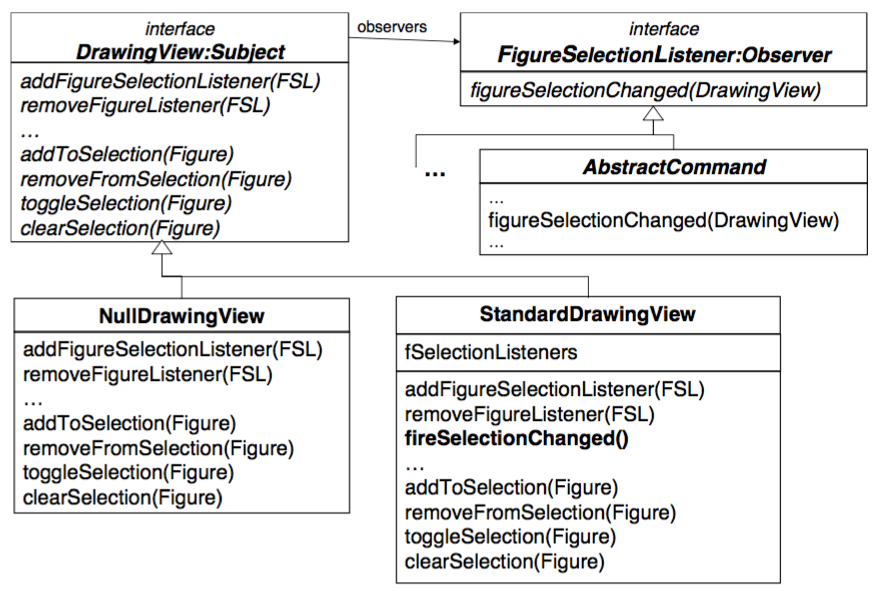
\includegraphics[width=.5\textwidth]{figures/BG_Observer_pattern_Selection_Listener.png}}
%   	\caption{Observer pattern: Selection Listener \cite{marin2005approach}}
%   	\label{fig:Selection_Listener}
% \end{figure}

% The \texttt{FigureSelectionListener} has the \textit{Observer} role in the pattern implementation. 
% Any class that is subject to changes of the selection of figures in a \texttt{DrawingView}, implements this interface. 
% The \texttt{DrawingView} interface partially defines the \textit{Subject} role by including two methods \texttt{addViewChangeListener} and \texttt{removeViewChangeListener}.
% From the classes that implement this interface only one, the \texttt{StandardDrawingView}, contains a non-empty implementation of the \textit{Subject} role in the \texttt{fireSelectionChanged} method.
% Note that this method is only defined in the concrete class, which deviates from the standard Observer pattern implementation.

% In their aspect refactoring, they described an aspect that is constructed comprising both the \textit{Subject} and \textit{Observer} roles definition and maintaining a list of associations between each \textit{Subject} and its \textit{Observer} objects.
% Their type-based refactoring\cite{marin2005approach} distinguishes several crosscutting elements in JHotDraw's \textit{Observer} pattern. 
% First, the role superimposition, applied twice, for each of the two roles. 
% Second, consistent behavior to notify the observers of the changes in the \textit{Subject} object.
% Where superimposition is defined as the aspect implementation of a specific role and consistent behavior as the aspect implementation of a \textit{consistent behavior} for a number of method elements that can be captured by a natural pointcut.
% The \texttt{GenericRole} (empty) interface documents the crosscutting type of role superimposition. 
% Specific roles, like \textit{Observer} and \textit{Subject} (\texttt{SelectionSubject}) extend the interface.
% These elements are shown in Figure \ref{fig:Concerns_Selection_Listener}.

% \begin{figure}[H]
% 	\centering
%   	\fbox{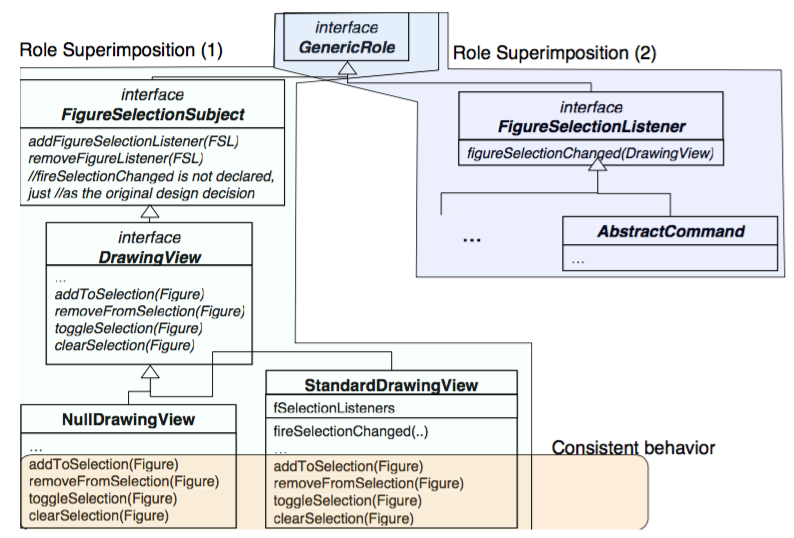
\includegraphics[width=.5\textwidth]{figures/BG_The_concern_types_in_Selection_Listener.png}}
%   	\caption{AJHotDraw: The concern types in Selection Listener \cite{marin2005approach}}
%   	\label{fig:Concerns_Selection_Listener}
% \end{figure}

% %%%%%%%%%%%%%%%%%%%%%%%%%%%%%%%%%%%%%%%%%%%%%%%%%%%%%%%%%%%
% \subsection{The ``Undo'' Concern of JHotDraw}\label{The Undo Concern of JHotDraw}
% Marin et al. have also identified the  ``Undo'' concern in JHotDraw. 
% A number of activities use this functionality including font sizes and colors, image rotation and a lot more.
% The authors propose the refactoring of the undo concern and more specifically a specific case the \textit{Change Attribute Command} \cite{marin2004refactoring}.

% A general representation of the elements in the JHotDraw implementation of the ``Undo'' concern can be seen in Figure \ref{fig:Participants_for_undo_in_JHotDraw}.

% \begin{figure}[H]
% 	\centering
%   	\fbox{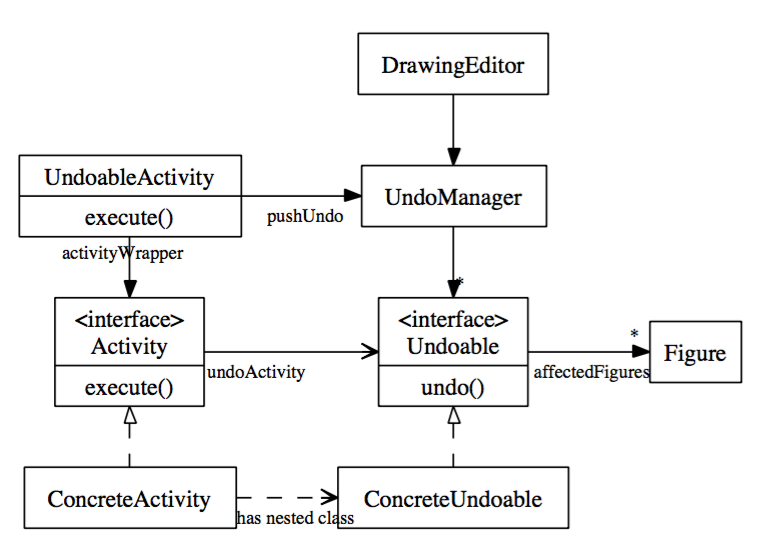
\includegraphics[width=.55\textwidth]{figures/BG_Participants_for_undo_in_JHOTDRAW.png}}
%   	\caption{Participants for undo in JHotDraw \cite{marin2004refactoring}}
%   	\label{fig:Participants_for_undo_in_JHotDraw}
% \end{figure}

% The \texttt{Activity} component participates in the implementation of the \textit{Command} design pattern\cite{gamma1995design}. 
% Many of these activities have support for undo functionality, which in JHotDraw is implemented by means of nested (undo) classes.
% The nested class knows how to undo the given activity which maintains a list of affected figures whose state is also affected if the activity would be ``undone''. 
% Whenever the activity modifies its state it also updates fields in its associated undo activity to actually perform the undo. 

% The implementation of AJHotDraw succeeded in refactoring this concern in JHotDraw through the following steps \cite{marin2004refactoring}:

% \begin{enumerate}

% 	\item An undo-dedicated aspect is associated to each of undo-able command. 
% 	The aspect will implement the entire undo functionality for the given command, while the undo code is removed from the command class.

%  	\item Each aspect will consistently be named by appending \texttt{UndoActivity} to the name of its associated command class to enforce the relation between the two.

% 	\item Next, the command's nested \texttt{UndoActivity} class moves to the aspect. 
% 	The factory methods for the undo activities also move to the the aspect, from where are introduced back, into the associated command classes, using inter-type declarations.

% 	\item Finally, the undo setup is attached to those methods from which was previously removed, namely execute() method, by means of an AspectJ \texttt{advice}.

% \end{enumerate}

% In particular, this proposition is applied in the \texttt{ChangeAttributeCommand} \cite{marin2004refactoring}.
% The undo \ac{ccc} has been identified, then removed from the system, and finally re-added in an aspect-specific manner.

% In this chapter we investigated both the \texttt{FigureSelectionListener} and the \texttt{ChangeAttributeCommand} (\textit{Undo}) concerns by refactoring them in a new version of the JHotDraw and compare them to their \ac{aop} counterpart.

%%%%%%%%%%%%%%%%%%%%%%%%%%%%%%%%%%%%%%%%%%%%%%%%%%%%%%%%%%%
\section{Crosscutting Concerns Identification}
Our managed data framework addresses the problem of \ac{ccc} by capturing them in modular data managers.
Yet, to solve the problem of \ac{ccc} it is first required to identify them in the source code.
This leads to a process called \textit{aspect mining}.
\textit{Aspect mining} is a reverse engineering process that aims at finding \ac{ccc} in existing systems \cite{marin2004identifying}.
The aspect mining topic has been addressed in previous research that include methods such as clone detection \cite{bruntink2005use}, machine learning \cite{shepherd2004design}, IDE tools \cite{robillard2002concern} and more. 
Marin et al. \cite{marin2004identifying} introduced a technique constructed by spotting methods that are invoked from many different places (high fan-in), in order to identify candidate aspects in open-source Java systems.
One of these projects include the JHotDraw.
In this thesis we focused on their concern findings in refactoring JHotDraw.
In particular, we focused on the \textit{FigureSelection}, concern, which is an observer pattern implementation.

\section{Aspect Refactoring in Managed Data}
In order to evaluate the ability of managed data to handle aspects, we have refactored two \ac{ccc} that have been identified in JHotDraw.
More specifically, in this chapter we present the refactoring of the \textit{FigureSelectionListener} observer pattern.
In this chapter we investigated both the \texttt{FigureSelectionListener} and the \texttt{ChangeAttributeCommand} (\textit{Undo}) \ac{ccc}.
The choice of those concerns has been made on purpose, since those are the concerns that AJHotDraw refactors using AspectJ and \ac{aop} techniques.
For the refactoring we used our implementation of managed data in Java, presented in the previous chapter.
Therefore, by having three versions of the same application (JHotDraw) and by solving the same concerns we will be able to perform a comparative evaluation.
The three systems included in our assessment are: \textbf{JHotDraw}\footnote{\url{http://www.jhotdraw.org/}}, the original \ac{oop} version, \textbf{AJHotDraw}\footnote{\url{https://sourceforge.net/projects/ajhotdraw/}}, the \ac{aop} refactored version and our \textbf{ManagedDataJHotDraw}\footnote{\url{https://github.com/TheolZacharopoulos/ManagedDataJHotDraw}}, the managed data refactored version.
We focused on those concerns because they were also identified, solved, analyzed and presented in AJHotDraw.
Note that, for compatibility and comparison reliance, we used the version \textit{JHotDraw v.5.4b1} since AJHotDraw also refactors the same version.

In order to refactor JHotDraw, we first had to migrate it in managed data.
The result of this migration is available on an open-source project, the ManagedDataJHotDraw.
We claim that this is the first aspect refactoring of an application using managed data to date, since this project aims on showing how managed data can deal with \ac{ccc} in existing systems.

\section{Migration Process}\label{Migration}
The refactoring of an application of JHotDraw's size required a significant amount of time to study and familiarize with, yet, its well-designed \ac{oop} code, made it easy to grasp.
We solely focused on the parts that were going to be refactored, based on refactorings that AJHotDraw developers \cite{marinajhotdraw} performed.
Thanks to their fan-in analysis \cite{marin2004identifying}, we targeted the same concerns in order to make a fair comparison.
Furthermore, during the implementation of ManagedDataJHotDraw we focused on maintaining behavioral coherence and the original design.
The migration process of the basic components is detailed described in Appendix \ref{Migration Process}.

%%%%%%%%%%%%%%%%%%%%%%%%%%%%%%%%%%%%%%%%%%%%%%%%%%%%%%%%%%%
\section{Aspect Refactoring of JHotDraw}
Aspect refactoring usually refers to the refactoring of legacy code in aspect oriented code. 
However, in this section we present an aspect refactoring of JHotDraw legacy code in managed data.

%%%%%%%%%%%%%%%%%%%%%%%%%%%%%%%%%%%%%%%%%%%%%%%%%%%%%%%%%%%
% FigureSelectionListener
%%%%%%%%%%%%%%%%%%%%%%%%%%%%%%%%%%%%%%%%%%%%%%%%%%%%%%%%%%%
\section{FigureSelectionListener: Observer Pattern}
The \texttt{FigureSelectionListener} observer pattern of JHotDraw is a concern first presented by Hannemann et al. \cite{hannemann2005role} in their role-based refactoring of design patterns in AspectJ. 
Later, Marin et al. used the same concern and migrated it into their AJHotDraw implementation \cite{marin2005approach}.
Likewise, we have also implemented the same aspect for our refactoring in order to compare our aspect solution with the existing one.

\subsection{FigureSelectionListener in JHotDraw}
The original \texttt{FigureSelectionListener} observer pattern of JHotDraw is illustrated in Figure \ref{fig:JHotDraw_FigureSelectionListener_OOP}.

\begin{figure}[H]
	\centering
  	\fbox{\includegraphics[width=1\textwidth]{figures/JHotDraw_FigureSelectionListener_OOP.png}}
  	\caption{FigureSelectionListener in JHotDraw}
  	\label{fig:JHotDraw_FigureSelectionListener_OOP}
\end{figure}

As this figure illustrates, the \texttt{FigureSelectionListener} interface defines the \textit{Observer} role.
The classes that are interested in the changes of selection of figures in a \texttt{DrawingView} implement this interface.
Accordingly, the \texttt{DrawingView} defines the \textit{Subject} role, providing methods for adding and removing figure selection listeners.
Practically, the only class that implements the \textit{Subject} role is \texttt{StandardDrawingView}, while \texttt{NullDrawingView} has an empty implementation.

\texttt{StandardDrawingView} keeps the selection listeners in a list, the \texttt{fSelectionListeners}, and notifies them in the invocation of the \texttt{fireSelectionChanged} method.
This method is called in the methods: \texttt{addToSelection}, \texttt{removeFromSelection}, \texttt{toggleSelection} and \texttt{clearSelection}, which indicate the change of figure selection.
On the observers' side, the figure selection listeners implement the \texttt{figureSelectionChanged} method that is executed in case they have been notified by the subject.

Concluding, as described above, the ``pattern code'' of the observer pattern is scattered in many places, including the list of listeners on the subject, the add / remove methods, along with the pointcut methods that call the method which notifies the listeners.

%%%%%%%%%%%%%%%%%%%%%%%%%%%%%%%%%%%%%%%%%%%%%%%%%%%%%%%%%%%%%
\subsection{Refactoring FigureSelectionListener in AJHotDraw}
Marin et al. presented a refactoring of this concern in AJHotDraw \cite{marin2005approach}. 
Their refactoring is illustrated in Figure \ref{fig:JHotDraw_FigureSelectionListener_AOP}. 

\begin{figure}[H]
	\centering
  	\fbox{\includegraphics[width=.8\textwidth]{figures/JHotDraw_FigureSelectionListener_AOP.png}}
  	\caption{FigureSelectionListener in AJHotDraw}
  	\label{fig:JHotDraw_FigureSelectionListener_AOP}
\end{figure}

In their proposed type-based refactoring, they have used two crosscut sorts, namely \textit{role superimposition} and \textit{consistent behavior}.

\subsubsection{Role Superimposition}
As defined by the authors \cite{marin2005classification}, ``the role superimposition refers to the implementation of a specific secondary role or responsibility''.
In the case of \texttt{FigureSelectionListener}, they used it twice, one for each of the roles.
More specifically, they defined an abstract \texttt{GenericRole} and concrete roles, observer and subject which extend the abstract one.

\subsubsection{Consistent Behavior}
According to the authors\cite{marin2005classification}, ``the consistent behavior sort implements a consistent behavior for a number of method elements that can be captured by a natural pointcut''.
In this case it is used to notify the \textit{Observers} of the changes in the \textit{Subject} object.
More specifically, the methods \texttt{addToSelection}, \texttt{removeFromSelection}, \texttt{toggleSelection} and \texttt{clearSelection} are consistent behavior.
They implement it as a pointcut in AspectJ shown in Listing \ref{lst:Consistent Behavior in FigureSelectionListener}.

\begin{sourcecode} [H]
	\begin{lstlisting}[language=AspectJ]
public aspect SelectionChangedNotification {
	pointcut invalidateSelFigure(StandardDrawingView sdw) :
		(   withincode(boolean StandardDrawingView.addToSelectionImpl(Figure)) 
		 || withincode(void StandardDrawingView.removeFromSelection(Figure)))
		&& call(void Figure.invalidate()) 
		&& this(sdw);

	pointcut clear_toggleSelection(StandardDrawingView sdw):
		(execution(void StandardDrawingView.clearSelection()) ||
		 execution(void StandardDrawingView.toggleSelection(Figure)))
		&& this(sdw);

	after(StandardDrawingView sdw): invalidateSelFigure(sdw) {
		sdw.fireSelectionChanged();
	}

	after(StandardDrawingView sdw): clear_toggleSelection(sdw) {
		sdw.fireSelectionChanged();
	}
}
	\end{lstlisting}
	\caption{AJHotDraw: Consistent Behavior in FigureSelectionListener}
	\label{lst:Consistent Behavior in FigureSelectionListener}
\end{sourcecode}

\subsubsection{Benefits and Limitations}
According to the authors \cite{marin2005approach}, such refactoring allows the crosscutting elements to be addressed individually, which leads to a modular solution, and any deviations from the pattern implementation can be addressed separately.

However, as they mention, the definition of pointcuts in order to capture the calls to the notifier is difficult when many consistent behavior instances occur. 
As Listing \ref{lst:StandardDrawingView clearSelection Method} shows, the original \texttt{clearSelection} method in JHotDraw calls \texttt{fireSelectionChanged} under specific conditions.
Considering the \ac{aop} solution of AJHotDraw, Listing \ref{lst:Consistent Behavior in FigureSelectionListener}, this is not the case.
In the pointcut definition, the pattern refactoring solution notifies the observers independently of the condition in the caller.
Although, according to Marin et al. it is potentially harmless in this case, this implementation deviates from the behavior of the original JHotDraw, leading to a harmful, for the functionality, implementation.
Finally, the problem of the unconditional call of a method in a pointcut is clearly a problem of the language.
AspectJ mechanisms do not support such functionality.
But can managed data solve this problem?

\begin{sourcecode}
	\begin{lstlisting}[language=AspectJ, escapechar=|]
public void clearSelection() {
	if (selectionCount() == 0) {
		// avoid unnecessary selection changed event when nothing has to be cleared
		return;
	}
	FigureEnumeration fe = selection();
	while (fe.hasNextFigure()) {
		fe.nextFigure().invalidate();
	}
	...
	fireSelectionChanged();
}
	\end{lstlisting}
	\caption{StandardDrawingView clearSelection Method}
	\label{lst:StandardDrawingView clearSelection Method}
\end{sourcecode}

%%%%%%%%%%%%%%%%%%%%%%%%%%%%%%%%%%%%%%%%%%%%%%%%%%%%%%%%%%%%%
\subsection{Refactoring FigureSelectionListener in ManagedDataJHotDraw}
In JHotDraw's original code, the \textit{observer} \texttt{DrawApplication} creates a new \texttt{StandardDrawingView} instance using the \texttt{createDrawingView} method.
During the construction the \texttt{DrawApplication} passes itself to the constructor of the \texttt{StandardDrawingView} and this in turn adds it to its listeners list, using the \texttt{addFigureSelectionListener} method.
This is shown in Line \ref{line:addFigureSelectionListener_contructor} of Listing \ref{lst:DrawingView Constructor}.
Likewise, the rest of the classes that implement the \texttt{FigureSelectionListener} interface, perform the same mechanism, adding or removing themselves from the \texttt{DrawingView} \textit{Subject}.
Consequently, the pattern code is scattered among its participants.

In this section we present our managed data refactoring of the \texttt{FigureSelectionListener} concern.
Managed data implements aspects using data managers, by adding specifications to the data.
For this case, we needed a similar mechanism to the \textit{role superimposition} of \ac{aop}.
This mechanism should be defined in a data manager that will produce managed data instances (managed objects) with a specific role.
Additionally, the data manager has to support something similar to the \textit{consistent behavior} as a pointcut.

In detail, since the \texttt{DrawingView} is managed data, and it is the \textit{Subject} to the \textit{Listeners} of the \textit{FigureSelectionListener} case, we can implement a data manager that attaches the \textit{Subject} \texttt{MDStandardDrawingView}.
Therefore, no \textit{Subject} role specific code will be tangled with the \texttt{DrawingView}, but a data manager will attach this role later.

More specifically, we needed a data manager that performs the following:

\begin{enumerate}
	\item Attaches the \textit{Subject} role to the \texttt{MDStandardDrawingView} since this object implements the pattern.
	Initially, \texttt{MDStandardDrawingView} has no \textit{Subject} role related code.

	\item Enables the \textit{Subject} to \textit{add} and \textit{remove} listener objects to and from itself. 
	\newline
	In this case the \texttt{FigureSelectionListener} instances.

	\item Defines an \textit{Action} that will be executed on the listeners in case of the \textit{Subject}'s notification.
	\newline
	In this case the \texttt{figureSelectionChanged} method.

	\item Finally, it defines a pointcut for the consistent behavior that executes the actions on the listeners. 
	In this case the \texttt{addToSelection}, \texttt{removeFromSelection}, \texttt{toggleSelection} and \texttt{clearSelection} methods.
\end{enumerate}

\subsubsection{Data manager}
First, we can abstract the \textit{Subject} role concern code in a separate data manager.
As it is mentioned in Chapter \ref{Implementation}, the role of a data manager class is to create a \texttt{MObject}, which interprets and handles a managed object instance.
Therefore, we first need this \texttt{MObject}, namely \texttt{SubjectRoleMObject}, to implement our subject role specifications.

\subsubsection{SubjectRole specifications}
We define the functionality of the \textit{SubjectRole} in an interface, shown in Listing \ref{lst:SubjectRole Interface}.
The subject role simply needs to add and remove listener objects to and from a managed object.
Additionally, it defined a method \texttt{executeListenerActions} that allows the subjects to execute all the actions of their listeners.

\begin{sourcecode} [H]
	\begin{lstlisting}[language=Java, escapechar=|]
public interface SubjectRole {
	void addListener(Object listener, Action action);
	void removeListener(Object listener);
	void executeListenerActions();
}
	\end{lstlisting}
	\caption{SubjectRole Interface}
	\label{lst:SubjectRole Interface}
\end{sourcecode}

\subsubsection{Action}
Additional to the listener object a \textit{SubjectRole} has to define an \textit{Action} for that listener.
That \textit{Action} determines the method which will be executed in that \textit{Listener} in case a notification is retrieved from the \textit{Subject}.
As Listing \ref{lst:Action Interface} shows, this is simply a functional interface that represents an executable action.

\begin{sourcecode} [H]
	\begin{lstlisting}[language=Java, escapechar=|]
@FunctionalInterface
public interface Action {
	void execute();
}
	\end{lstlisting}
	\caption{Action Interface}
	\label{lst:Action Interface}
\end{sourcecode}

\subsubsection{SubjectRole MObject}
Having the specifications of a Subject in place we need a data manager that implements them.
This data manager defines a ``role superimposition'' of the subject role.

\paragraph{Role Superimposition}\mbox{}\\
The implementation of the \texttt{SubjectRoleMObject} is presented in Listing \ref{lst:SubjectRoleMObject}.
First, the SubjectRoleMObject extends the MObject, inheriting the functionalities of the base data manager, followed by the implementation of the \texttt{SubjectRole} specifications.
By implementing the \texttt{SubjectRole} interface, the MObject has to implement the \texttt{addListener} and \texttt{removeListener} methods that have been provided by the subject role specifications.
Having added a listener object along with its \texttt{Action} to be executed on each notification, the method \texttt{executeListenerActions} executes all the actions for each of the listeners.

\begin{sourcecode} [H]
	\begin{lstlisting}[language=Java, escapechar=|]
public class SubjectRoleMObject extends MObject implements SubjectRole { |\label{line:subj_mobj_extends}|
	protected Map<Object, Action> listeners;
	public SubjectRoleMObject(Klass schemaKlass, Object... initializers) {
		super(schemaKlass, initializers);
		listeners = new HashMap<>();
	}
	public void executeListenerActions() {
		listeners.values().forEach(Action::execute); |\label{line:subj_mobj_execute}|
	}
	public void addListener(Object listener, Action action) {
		listeners.put(listener, action);
	}
	public void removeListener(Object listener) {
		listeners.remove(listener);
	}
}
	\end{lstlisting}
	\caption{SubjectRoleMObject}
	\label{lst:SubjectRoleMObject}
\end{sourcecode}

\subsubsection{Consistent Behavior}
Since we have implemented a form of \textit{role superimposition} what is left is the \textit{consistent behavior} pointcut.
However, this functionality is application specific, therefore we can extend the abstract \texttt{SubjectRole} data manager with an application specific data manager that implements the consistent behavior.
For practical reasons, we used an interface to define these specifications.
As Listing \ref{lst:FigureSelectionPointcut} shows, a list of the methods that execute the \texttt{Action} for each listener are defined in the \texttt{FigureSelectionPointcut} interface. 

\begin{sourcecode} [H]
	\begin{lstlisting}[language=Java, escapechar=|]
public interface FigureSelectionPointcut {
	void addToSelection(Figure figure);
	void removeFromSelection(Figure figure);
	void toggleSelection(Figure figure);
	void clearSelection();
}
	\end{lstlisting}
	\caption{FigureSelectionPointcut Interface}
	\label{lst:FigureSelectionPointcut}
\end{sourcecode}

\subsubsection{FigureSelectionListenerSubjectRole MObject}
Finally, having all of our specifications in place, we need to implement the actual MObject that uses them.
Of course we need a new data manager that is application specific, namely FigureSelectionListenerSubjectRole.
In particular, the FigureSelectionListenerSubjectRole MObject implements those specifications and provides its managed objects with the ability to use them.
Additionally, this data manager extends the \texttt{SubjectRole} data manager, creating a stack of data managers.
By stacking the data managers we have separated the application specific code, the consistent behavior in this case, from the more general subject role code.

\paragraph{Consistent Behavior Pointcut}\mbox{}\\
Considering that an MObject is an Invocation Handler, every method invocation passes through that object first.
By defining the pointcut in an interface and extending that interface in this MObject, we proxy the execution of the real object's methods, starting with MObject first.
This allows the programmer to add functionalities in these methods which in other cases would scatter the real object's methods.
Similarly to the \ac{aop} solution, the pointcut includes the three methods that call the \texttt{fireSelectionChanged} method.
However, in managed data, we are not limited to a specific method of a class but to an \texttt{Action} passed for the specific listener.
Invoking the \texttt{executeListenerActions} method on each of the methods defined by the pointcut, we have implemented the concern as a modular aspect.
Listing \ref{lst:FigureSelectionListenerSubjectRoleMObject} illustrates the code of the FigureSelectionListenerSubjectRole data manager.

\paragraph{Conditions in Pointcuts}\mbox{}\\
As it has been seen from the \ac{aop} solution, during the pointcut definition, the language did not allow to add any kind of conditions or other functionalities based on the state of the object.
However, since the MObject is proxied to a \texttt{MDStandardDrawingView} instance, the programmer can access the current state of the instance inside the data manager implementation.
Therefore, the programmer can use the state of the program.
In this case, the execution of the action on the listener is performed under a specific condition, (Line \ref{line:fig_lis_mobj_clear} of Listing \ref{lst:FigureSelectionListenerSubjectRoleMObject}), which is similar to the one defined on the original program \ref{lst:StandardDrawingView clearSelection Method}.

\begin{sourcecode} [H]
	\begin{lstlisting}[language=Java, escapechar=|]
public class FigureSelectionListenerSubjectRoleMObject 
	extends SubjectRoleMObject implements FigureSelectionPointcut {

	public FigureSelectionListenerSubjectRoleMObject(
		Klass schemaKlass, Object... initializers) 
	{
		super(schemaKlass, initializers);
	}

	@Override
	public void addToSelection(Figure figure) {
		executeListenerActions();
	}

	@Override
	public void removeFromSelection(Figure figure) {
		executeListenerActions();
	}

	@Override
	public void toggleSelection(Figure figure) {
		executeListenerActions();
	}

	@Override
	public void clearSelection() {
		if (((MDStandardDrawingView) thisObject).selectionCount() > 0) { |\label{line:fig_lis_mobj_clear}|
			executeListenerActions();
		}
	}
}
	\end{lstlisting}
	\caption{FigureSelectionListenerSubjectRoleMObject}
	\label{lst:FigureSelectionListenerSubjectRoleMObject}
\end{sourcecode}

\begin{figure} [H]
	\centering
  	\fbox{\includegraphics[width=1\textwidth]{figures/JHotDraw_FigureSelectionListener_MD.png}}
  	\caption{FigureSelectionListener in ManagedDataJHotDraw}
  	\label{fig:JHotDraw_FigureSelectionListener_MD}
\end{figure}

\subsection{Managed Data Refactoring}
Figure \ref{fig:JHotDraw_FigureSelectionListener_MD} illustrates the refactored version of the FigureSelectionListener concern in ManagedDataJHotDraw.
Comparing it to the original, Figure \ref{fig:JHotDraw_FigureSelectionListener_OOP}, it can be seen that, first, the list of listeners has been removed from the \texttt{DrawingView}. 
Next, the \texttt{addListener} and \texttt{removeListener} methods have also been removed from the class.
Every call of the \texttt{fireSelectionChanged} method in the pointcut methods has also been omitted.
Finally, conditions on the pointcuts have been defined, something that is not supported by the \ac{aop} version, AJHotDraw.

The integration of the data manager was executed simply by using our schema factories and adding the listeners during construction.
Most importantly, the behavior of the application remained equivalent to the original.
ManagedDataJHotDraw conserved the behavior of JHotDraw, which we evaluated through its own test suite along with manual tests.
Interestingly, by stacking data managers we manage to define aspects of our data in a modular way.

%%%%%%%%%%%%%%%%%%%%%%%%%%%%%%%%%%%%%%%%%%%%%%%%%%%%%%%%%%%%%%%%%%%%%%%%%%%%%%%
% Undo Concern
%%%%%%%%%%%%%%%%%%%%%%%%%%%%%%%%%%%%%%%%%%%%%%%%%%%%%%%%%%%%%%%%%%%%%%%%%%%%%%%
\section{ChangeAttributeCommand: Undo Concern}
The ``Undo'' functionality is used in several places in the original JHotDraw.
Marin's fan-in analysis \cite{marin2004identifying}, identified about 30 undo activities defined for various elements of JHotDraw. 
For our assessment we focused on the refactoring of the undo concern in the \textit{ChangeAttributeCommand} class.
We choose the specific case since is the same that is used by Marin et al. on their undo refactoring in AJHotDraw \cite{marin2004refactoring}.

\subsection{ChangeAttributeCommand in JHotDraw}
The original Undo concern in \textit{ChangeAttributeCommand} of JHotDraw is illustrated in Figure \ref{fig:JHotDraw_Undo_Command_ChangeAttributeCommand_OOP}.

\begin{figure} [H]
	\centering
  	\fbox{\includegraphics[width=0.6\textwidth]{figures/JHotDraw_Undo_Command_ChangeAttributeCommand_OOP.png}}
  	\caption{ChangeAttributeCommand in JHotDraw}
  	\label{fig:JHotDraw_Undo_Command_ChangeAttributeCommand_OOP}
\end{figure}

A command of the \textit{Command} pattern is represented by the \texttt{Command} interface in the figure. 
Some of the activities support the undo functionality, which is implemented in nested \texttt{UndoActivity} classes.

In the case of the \textit{ChangeAttributeCommand}, the command is called when an attribute is applied to a figure.
An attribute can be a color, a font, a url etc.
When an attribute has been applied using a \textit{ChangeAttributeCommand} object, the object defines its \texttt{UndoActivity} through the \textit{UndoActivity} private class.

The role of the \texttt{UndoableCommand} wrapper class is to support repeated undo operations since it records the last executed commands of the wrapper class, in reverse order.
In particular, this class acquires a reference to the undo activity associated with the wrapped command and it pushes it into a stack managed by an \texttt{UndoManager} \cite{marin2004refactoring}.

Therefore, as Marin et al. concluded \cite{marin2004identifying} the ``Undo'' concern code is scattered in several places of the Command classes.
First, the \texttt{myUndoableActivity} field in the \texttt{AbstractCommandClass} along with its accessors, \texttt{getUndoActivity} and \texttt{setUndoActivity}.
Next, the private nested classes are implemented by the concrete commands that support undo.
Moreover, the factory method, \texttt{createUndoActivity} creates instances of the private classes.
Finally, the references to the before enumerated elements from non-undo related members.

\subsection{Refactoring ChangeAttributeCommand in AJHotDraw}
The refactoring that Marin et al. proposed can be seen in Figure \ref{fig:JHotDraw_Undo_Command_ChangeAttributeCommand_AOP}.

\begin{figure} [H]
	\centering
  	\fbox{\includegraphics[width=0.65\textwidth]{figures/JHotDraw_Undo_Command_ChangeAttributeCommand_AOP.png}}
  	\caption{ChangeAttributeCommand in AJHotDraw}
  	\label{fig:JHotDraw_Undo_Command_ChangeAttributeCommand_AOP}
\end{figure}

As the figure shows, a new aspect is created for the \textit{ChangeAttributeCommand}.
In this aspect the entire undo functionality is implemented and the undo code is removed from the actual \textit{ChangeAttributeCommand} class. 
Additionally, the private class that implements the \textit{UndoActivity} has moved to this aspect along with its factory method (\textit{createUndoActivity}).

However, by convention, each aspect will consistently be named by appending ``UndoActivity'' to the name of its associated command class, to enforce the relation between the two.
All the abstract undo functionality has been defined in a \textit{CommandUndo} aspect.
This aspect defines the undo as a role, the \textit{Undoable} field and its accessors of the \textit{AbstractCommand}.

Additionally, the change of the visibility of the methods introduced from the aspects is an issue.
The visibility declared in the aspect refers to the aspect and not to the target class. 
However, the same problem occurs in managed data.

\subsection{Refactoring ChangeAttributeCommand in ManagedDataJHotDraw}
Finally, the aspect refactoring of the \texttt{ChangeAttributeCommand} undo concern in JHotDraw using managed data is presented in Figure \ref{fig:JHotDraw_Undo_Command_ChangeAttributeCommand_MD}.

\begin{figure} [H]
	\centering
  	\fbox{\includegraphics[width=1\textwidth]{figures/JHotDraw_Undo_Command_ChangeAttributeCommand_MD.png}}
  	\caption{ChangeAttributeCommand in ManagedDataJHotDraw}
  	\label{fig:JHotDraw_Undo_Command_ChangeAttributeCommand_MD}
\end{figure}

To implement aspects using data managers in the \texttt{ChangeAttributeCommand} we first needed to migrate the original class to a managed data definition, namely \textit{MDChangeAttrCmd}.
The process was similar to the one described in Section \ref{Migration}.

In order to refactor the undo concern in managed data we needed a number of specifications that define the functionalities of our managed objects.
As the \ac{aop} solution shows we needed something similar to \textit{role superimposition}, but this time for the \textit{Undoable} role.
Additionally, we needed a way to define executables since our participant, in particular \texttt{ChangeAttributeCommand}, is a command.

In detail we needed a data manager that performs the following:
\begin{enumerate}
	
	\item Attaches an \textit{UndoableRole} to command instances.
	In this case the \texttt{MDChangeAttrCmd} instances.

	\item Following the original design, this role should allow the objects to create their \texttt{UndoActivities} using a nested private class.
	\textit{UndoableRole} should also provide accessors for its \textit{UndoActivity}.

	\item It defines an \textit{Executable} specification, since every command has an \texttt{execute} method.

	\item Finally, it defines a pointcut on the \texttt{execute} method since this is the place where the undo functionality for a specific command is implemented.

\end{enumerate}

\subsubsection{Data Manager}
First, for abstraction's sake we have implemented the \texttt{UndoableRole} interface to an abstract class, namely \texttt{UndoableRoleMObject}.
This data manager defines a \texttt{myUndoableActivity} field and implements its accessors given by the \texttt{UndoableRole} interface, including both \texttt{setUndoActivity} and \texttt{getUndoActivity}.
However, no implementation for the \texttt{createUndoActivity} factory method is provided at this point.
The reason is that this is a ``command-specific'' implementation and it has to be provided by the concrete classes.
Since this is an abstract \texttt{MObject} no proxy factory is provided (data manager).

Next, we needed a \texttt{MObject} for the concrete command, in this case the \texttt{UndoableChangeAttrCmdMObject}.
Since this has to inherit the \texttt{UndoableMObject}, it also has to implement the \texttt{createUndoActivity} method.
As mentioned, this is ``command-specific'' code, and following the original design, this functionality can be implemented in a nested class.
As a result, an \texttt{UndoActivity} private nested class is defined in the \texttt{UndoableChangeAttrCmdMObject} class file.
Instances of this class can be created using the \texttt{createUndoActivity} method.

Furthermore, the command is an executable object; therefore, this \texttt{MObject} has to implement the \texttt{Executable} interface.
By doing so, the pointcut of the specific undo functionality can be implemented inside this \texttt{execute} method of the \texttt{UndoableChangeAttrCmdMObject}.
A comparison of the \texttt{execute} method between the original and the refactored code can be seen in Listings \ref{lst:original_execute_undo} and \ref{lst:refactored_execute_undo}.
\newline
\lstdefinestyle{smallJava}{
  basicstyle={\scriptsize\ttfamily},
  language=Java
}

\noindent\begin{minipage}{.45\textwidth}
\begin{lstlisting}[
	style=smallJava,
	caption=Original execute method,
	frame=tlrb,
	label=lst:original_execute_undo
]
public void execute() {
	setUndoActivity(createUndoActivity());
	getUndoActivity()
		.setAffectedFigures(view().selection());
	FigureEnumeration fe = 
	  	getUndoActivity().getAffectedFigures();
	while (fe.hasNextFigure()) {
		fe.nextFigure().setAttribute(fAttribute, fValue);
	}
	view().checkDamage();
}
\end{lstlisting}
\end{minipage}\hfill
\begin{minipage}{.45\textwidth}
\begin{lstlisting}[
	style=smallJava,
	caption=Refactored execute method,
	frame=tlrb,
	label=lst:refactored_execute_undo
]
default void execute() {
	FigureEnumeration fe = view().selection();
	while (fe.hasNextFigure()) {
		fe.nextFigure().setAttribute(attribute(),value());
	}
	view().checkDamage();
}
	\end{lstlisting}
\label{lst:execute_undo}
\end{minipage}

As the two listings show, all of the \textit{Undo} related functionalities of the \texttt{ChangeAttributeCommand} command have been removed from the \texttt{execute} method.
This code is located at \texttt{UndoableChangeAttrCmdMObject} and more specifically at its execute pointcut.
Listing \ref{lst:The execute Undo pointcut} shows the pointcut code.

\begin{sourcecode}
	\begin{lstlisting}[language=Java]
public void execute() {
	setUndoActivity(createUndoActivity());
	getUndoActivity().setAffectedFigures(thisObj.view().selection());
}
public Undoable createUndoActivity() {
	return new UndoActivity(thisObj.view(), thisObj.attribute(), thisObj.value());
}
    \end{lstlisting}
	\caption{The execute Undo pointcut}
	\label{lst:The execute Undo pointcut}
\end{sourcecode}

\subsection{Managed Data Refactoring}
Comparing the original version with our refactored version several improved points can be observed.
First, all of the \textit{Undo} related functionalities of a command have been removed from the command's code and they have been externally attached by the \textit{UndoRole} data manager.
Next, following the original design, the creation of an \texttt{UndoActivity} instance is again defined inside a nested class; however, this time it is not in the command itself but it is inside a ``command-specific'' data manager.
Finally, the \texttt{execute} method of a command is not aware of its undo functionality since it has been extracted to an undo dedicated pointcut inside a data manager.

%%%%%%%%%%%%%%%%%%%%%%%%%%%%%%%%%%%%%%%%%%%%%%%%%%%%%%%%%%%%%
% Metrics
%%%%%%%%%%%%%%%%%%%%%%%%%%%%%%%%%%%%%%%%%%%%%%%%%%%%%%%%%%%%%
\section{Metrics}\label{Evaluation Metrics}
Concluding we have presented a new version of JHotDraw, the ManagedDataJHotDraw which refactors two \ac{ccc} of the original system.
We ensure that the new version preserved behavioral equivalence with the original, using the provided automated tests suite and manual tests.
However, to present the relation between the original and our implementation we have collected a set of metrics \cite{sant2003reuse}.

\subsection{Metrics Collection Details}\label{Metrics Collection Details}
First, those metrics measure the \textit{Size}, which can show to what extend our version changed the original in terms of the size factor.
Second, they measure \textit{Cohesion} and \textit{Coupling}, which shows how hard it is to understand, reuse and maintain the program.
Finally, they measure \textit{Separation of Concerns}, which presents the degree of scattering and tangling of the application .
The \textit{Separation of Concerns} metric is the most crucial for our research since this is the main criterion that we have focused on this refactoring.

For each concern refactoring on each system, we chose to collect data only for the participant classes so that our version would be comparable with the original.
If all classes were included our results would be inflated strictly due to the higher number of classes.
In addition, in the case of managed data, the abstract and reusable data manager classes have not been considered, i.e. the \texttt{SubjectRoleMObject} data manager.
The reason is that the data managers are reusable code and independent from the application's logic.
Certainly, any (low level) data managers that are application-specific, like the point-cut data managers, are measured, i.e. the \texttt{FigureSelectionListenerMObject}.

The metrics \ac{woc}, \ac{cbc}, \ac{lcoo} and \ac{dit} are similar to Chidamber and Kemerer's metrics and easy to be collected using simple software analysis tools.
Likewise, these tools can easily measure \ac{loc}, in our case we have used the \ac{ncloc} for reliability.

The \ac{noa} metric counts the attributes of a class.
The number of attributes in both \ac{oop} and \ac{aop} systems it is simply the number of fields.
However, \ac{noa} in the managed data system has a significant difference.
In managed data schema definitions everything is method declarations, even the fields; therefore, in order to count \ac{noa} we need to count the method declarations which are not \texttt{default} and therefore represent field declarations.

% #important
Finally, note that no data have been collected for the AJHotDraw version but only for the original JHotDraw and the managed data version, MDJHotDraw.
The reason is that, although those metrics support aspect abstractions in their definition \cite{sant2003reuse}, the comparison is not well-grounded.
Establishing reliable comparison between programs written in Java and programs written in AspectJ (and Java), could be misleading.
Because those languages differ in their abstraction mechanisms.
JHotDraw and MDJHotDraw are both written in pure Java; using the same abstractions.
However, in managed data the design has been changed significantly and thus, we compare the two systems in order to show how this design refactoring affects the original implementation.

\subsection{Data Collection}
For the data collection we used the \texttt{MetricsReloaded} \footnote{
	\url{https://github.com/BasLeijdekkers/MetricsReloaded}}plug-in for IntelliJ IDE\footnote{\url{https://www.jetbrains.com/idea/}}.
Using this tool we managed to collect the following metrics\footnote{
	The tool uses different acronyms \cite{chidamber1994metrics} for the metrics: \ac{cbc} is CBO, \ac{woc} is \ac{wmc} and \ac{lcoo} is \ac{lcom}.
}: \ac{loc}, \ac{woc}, \ac{cbc}, \ac{lcoo} and \ac{dit}.
Table \ref{tbl:metrics} presents the metrics collected for the systems under evaluation.
The detailed results are presented in Appendix \ref{Metrics Results}. 
These results are discussed in the following chapter.

\begin{table} [H]
\resizebox{\textwidth}{!}{%
	\begin{tabular}{@{}clcccc@{}}
	\toprule
	\multicolumn{1}{l}{} & \multicolumn{1}{c}{} & \multicolumn{2}{c}{\textbf{ObserverPattern (FigureSelectionListener)}} & \multicolumn{2}{c}{\textbf{Undo (ChangeAttributeCommand)}} \\ \midrule
	 & \multicolumn{1}{c}{\textbf{Metrics}} & \textbf{JHotDraw} & \multicolumn{1}{c|}{\textbf{MDJHotDraw}} & \textbf{JHotDraw} & \textbf{MDJHotDraw} \\
	\multirow{3}{*}{SoC} & \multicolumn{1}{l|}{\textbf{CDC}} & 8 & \multicolumn{1}{c|}{4} & 5 & 3 \\
	 & \multicolumn{1}{l|}{\textbf{CDO}} & 21 & \multicolumn{1}{c|}{8} & 16 & 8 \\
	 & \multicolumn{1}{l|}{\textbf{CDLOC}} & 46 & \multicolumn{1}{c|}{6} & 32 & 12 \\
	\multirow{2}{*}{Coupling} & \multicolumn{1}{l|}{\textbf{CBC}} & 170 & \multicolumn{1}{c|}{184} & 128 & 128 \\
	 & \multicolumn{1}{l|}{\textbf{DIT}} & 18 & \multicolumn{1}{c|}{16} & 10 & 11 \\
	Cohesion & \multicolumn{1}{l|}{\textbf{LCOO}} & 75 & \multicolumn{1}{c|}{64} & 14 & 12 \\
	\multirow{4}{*}{Size} & \multicolumn{1}{l|}{\textbf{VS}} & 8 & \multicolumn{1}{c|}{10} & 5 & 5 \\
	 & \multicolumn{1}{l|}{\textbf{LOC}} & 1793 & \multicolumn{1}{c|}{1878} & 1052 & 1063 \\
	 & \multicolumn{1}{l|}{\textbf{NOA}} & 53 & \multicolumn{1}{c|}{53} & 29 & 27 \\
	 & \multicolumn{1}{l|}{\textbf{WOC}} & 383 & \multicolumn{1}{c|}{368} & 198 & 199 \\ \cmidrule(l){2-6} 
	\end{tabular}}
\caption{Metrics}
\label{tbl:metrics}
\end{table}

%%%%%%%%%%%%%%%%%%%%%%%%%%%%%%%%%%%%%%%%%%%%%%%%%%%%%%%%%%%%%
% Claims
%%%%%%%%%%%%%%%%%%%%%%%%%%%%%%%%%%%%%%%%%%%%%%%%%%%%%%%%%%%%%
% \section{Claims}
% We claim that our framework successfully performed aspect refactoring of the \texttt{FigureSelectionListener} concern in JHotDraw.
% Furthermore, it evolved the pointcut concept of \ac{aop} by adding conditions on them.
% This leads to a solution that focuses on behavior conservation, lost in the case of the \ac{aop} refactoring.
% Moreover, we claim that our framework also performed a successful aspect refactoring of the \texttt{ChangeAttributeCommand} undo concern in JHotDraw.
% Additionally, it solves the \ac{aop}'s problem of useing naming conventions for the nested classes.
% Finally, we have collected a set of metrics in order to assess our results and compare them with the original.
